\chapter{Design}\label{chap:design}

    Da wie bereits erwähnt, die Projekte \emph{"ITCS-Management"} und \emph{"ITCS"} bereits existierten, waren das grundlegende Design und die technische Architektur bereits vorgegeben.
    Dies umfasst sowohl Aspekte wie die Transaktionsverwaltung der Datenbank, als auch Elemente im Frontend, wie die Navigation zwischen den Seiten oder die Farbpalette.

\section{"ITCS-Management"}\label{sec:itcs-management-design}
    Im Projekt \emph{"ITCS-Management"} wurde eine Vielzahl an kleineren Aufgaben erledigt. Dabei handelte es sich um Blazor-Seiten, die meist nur Datenbank-Entitäten tabellarisch
    darstellen und beschränktes Editieren ermöglichen sollten. Im Bericht selbst wird auf diese Aufgaben, aufgrund ihrer repetitiven Natur, nicht weiter eingegangen. Fokussiert wird  
    auf die größte Aufgabe in diesem Projekt namens \emph{"Umlaufeditor"}. 
    Ein Umlauf stellt dabei eine Sequenz von Fahrten dar, die von einem einzelnen Fahrzeug in einem Durchgang durchgeführt wird. Die Fahrten werden von den meisten Kunden in anderen 
    Systemen erstellt und sind mit dem Import neuer Versionen in der Datenbank schon vorhanden. Die Umläufe hingegen werden nicht in anderen Systemen definiert und sollen deswegen
    mit diesem Editor erstellt und angepasst werden. 
    \begin{figure}[H]
        \centering
        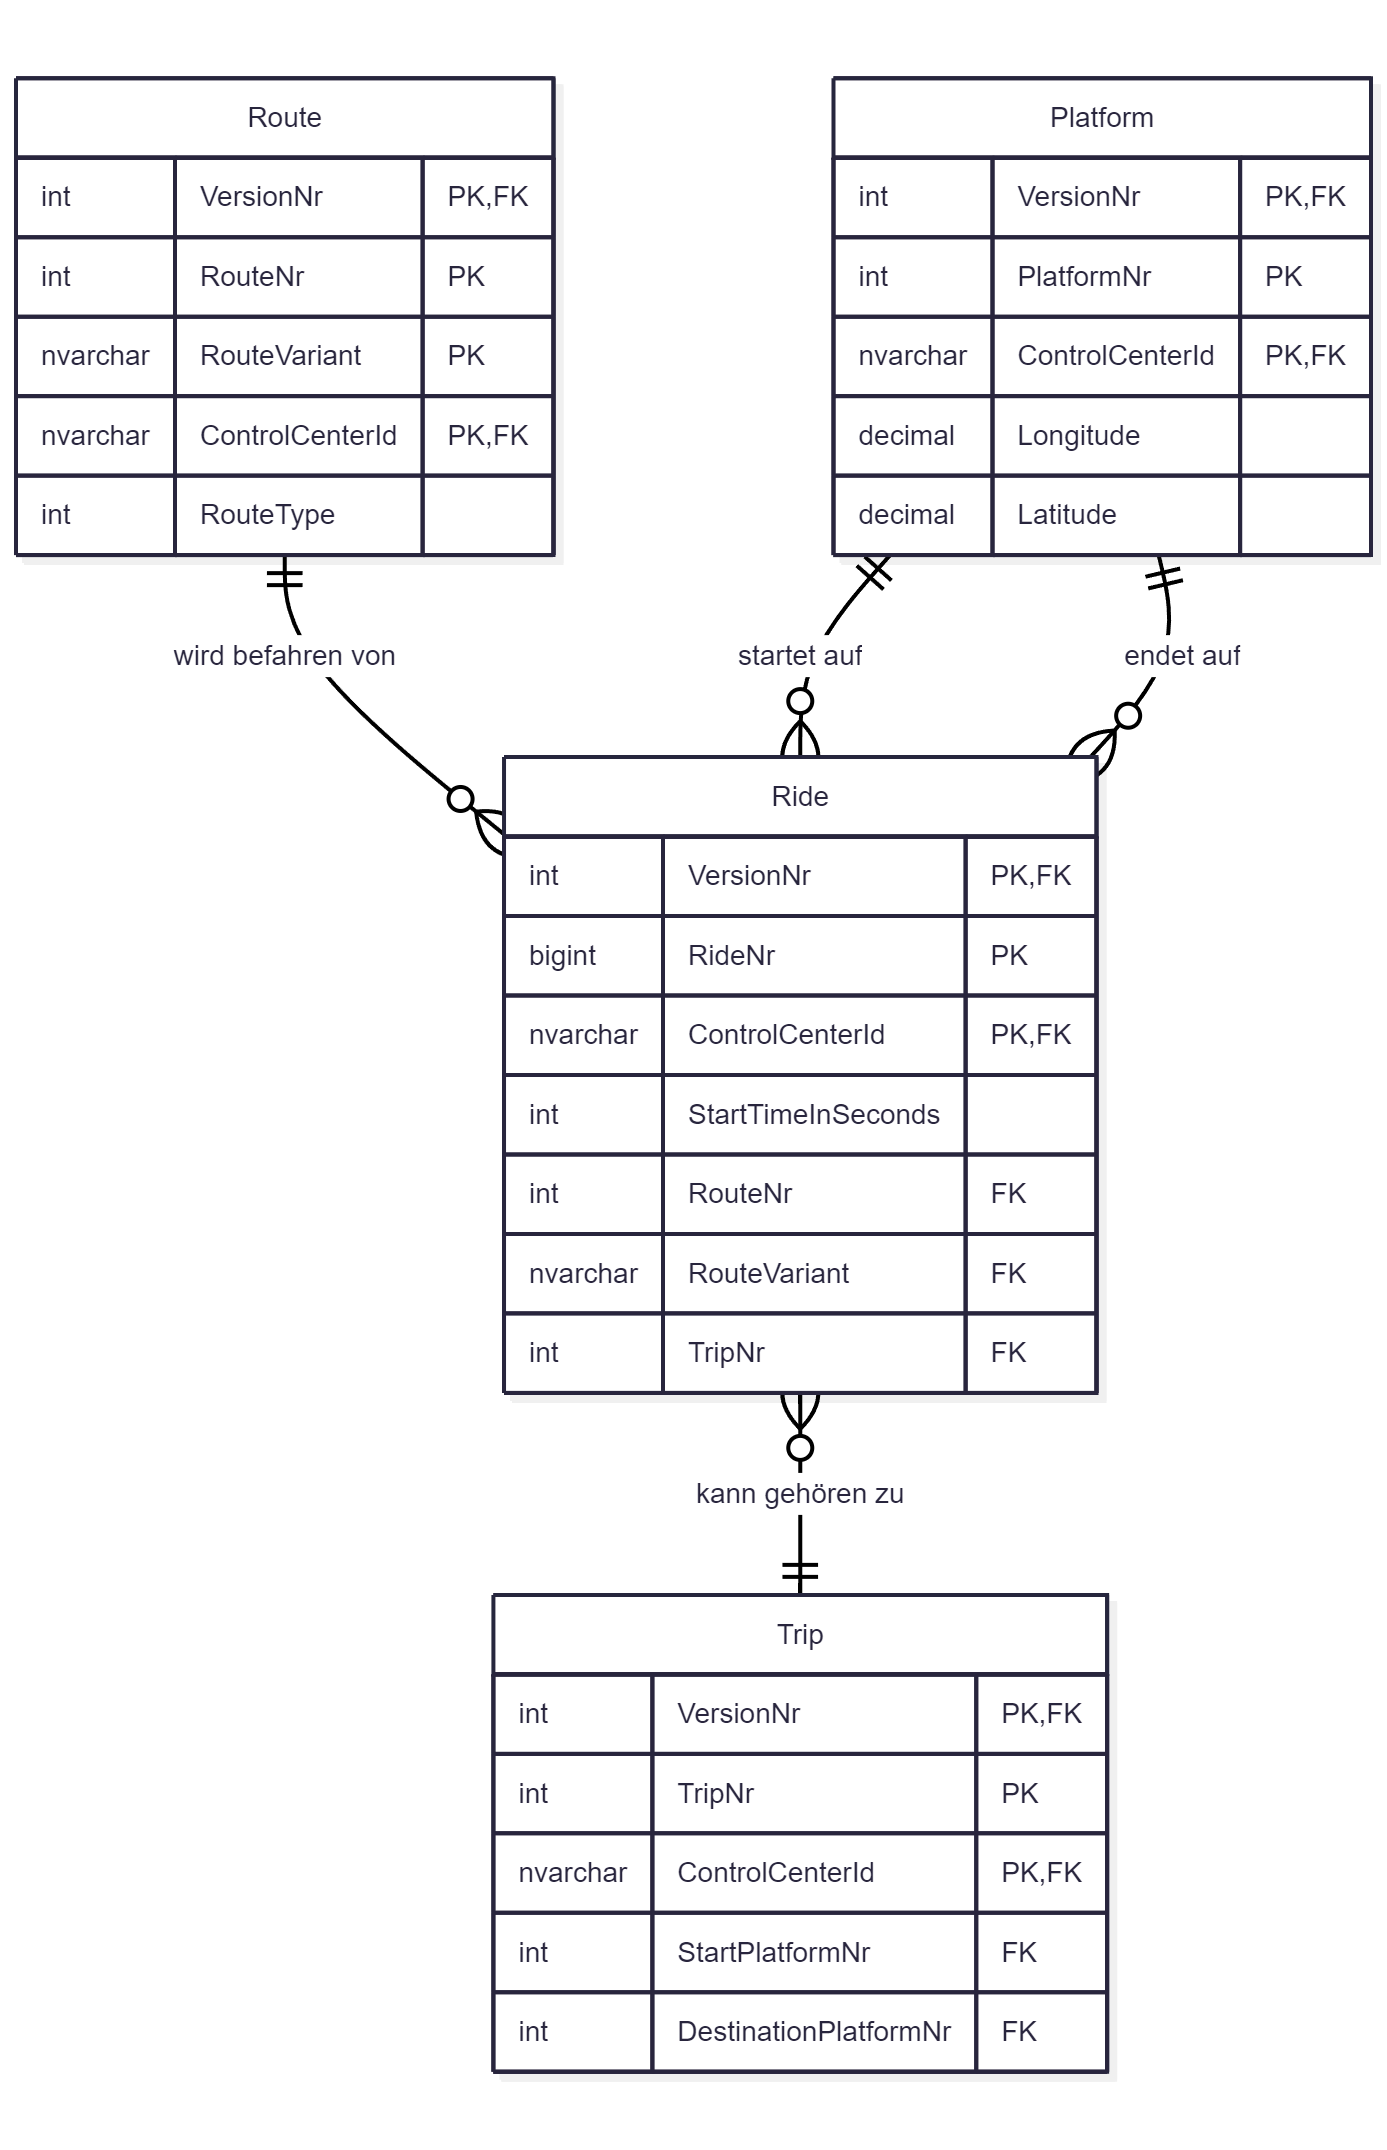
\includegraphics[width=0.8\textwidth]{transportation_system.png}
        \caption{Beziehungen von Umläufen und Fahrten}
        \label{fig:BeziehungenvonUmläufenundFahrten}
    \end{figure}

    Abbildung \ref{fig:BeziehungenvonUmläufenundFahrten} soll einen groben Überblick über das unmittelbar für diese Aufgabe benötigte Datenschema verschaffen. Für das Verständnis unwesentliche 
    Datenkomponenten und Beziehungen wurden weglassen. Die Entität "Route" ist in diesem Modell deswegen wichtig, da die Datenkomponente "RouteNr" die Art der Fahrt festlegt. Für Pausen oder nicht
    produktive
    Fahrten wird eine eigene Nummer vergeben. Zusätzlich ist bei jedem Umlauf ebenfalls jeweils eine Plattform-Entität (auch "Steig") als Start- und Endpunkt eingetragen. Dabei kann es sich bei den 
    Steigen um Sonderhaltepunkte wie beispielsweise Betriebshöfe handeln.

    Der Umlaufeditor besteht aus folgenden 3 Blazor-Seiten: 
    \begin{itemize}
        \item \emph{Sonderhaltepunkte}: Da Sonderhaltepunkte von den meisten Kunden nicht mit externen Tools erstellt werden und somit nicht beim Import neuer Versionen inbegriffen sind, 
                erlaubt diese Seite die Verwaltung und Erstellung neuer Sonderhaltepunkte.
        \item \emph{Umläufe}: Diese Seite stellt das Herzstück des Umlaufeditors dar. Hier können neue Umläufe erstellt und mit Fahrten versehen werden. Außerdem können bestehende Umläufe 
                als Vorlagen abgespeichert werden. 
        \item \emph{Vorlagen}: Hier können alle bestehenden Vorlagen eingesehen werden. Sollten für einen Umlauf mehrere Vorlagen bestehen oder Vorlagen in Zukunft nicht mehr durchführbar sein, können diese
                deaktiviert oder gelöscht werden.
    \end{itemize}

    Es sind zwar alle drei Seiten für den Einsatz des Umlaufeditors notwendig, jedoch verbirgt sich hinter der Seite \emph{Umläufe} die meiste Logik und sie stellt beim laufenden Betrieb das Herzstück dar.
    Der Prototyp der visuellen Grundstruktur der Seite ist in Abbildung \ref{fig:Umlaufeditor_konzept} zu sehen. Um die Seite implementieren zu können musste jedoch zunächst ein Konzept für den Ablauf 
    des Hinzufügens von Fahrten zu Umläufen erstellt werden. Das Ergebnis ist in vereinfachter Form als Ablaufdiagramms in Abbildung \ref{fig:Ablauf} zu sehen.

    \begin{figure}[H]
        \centering
        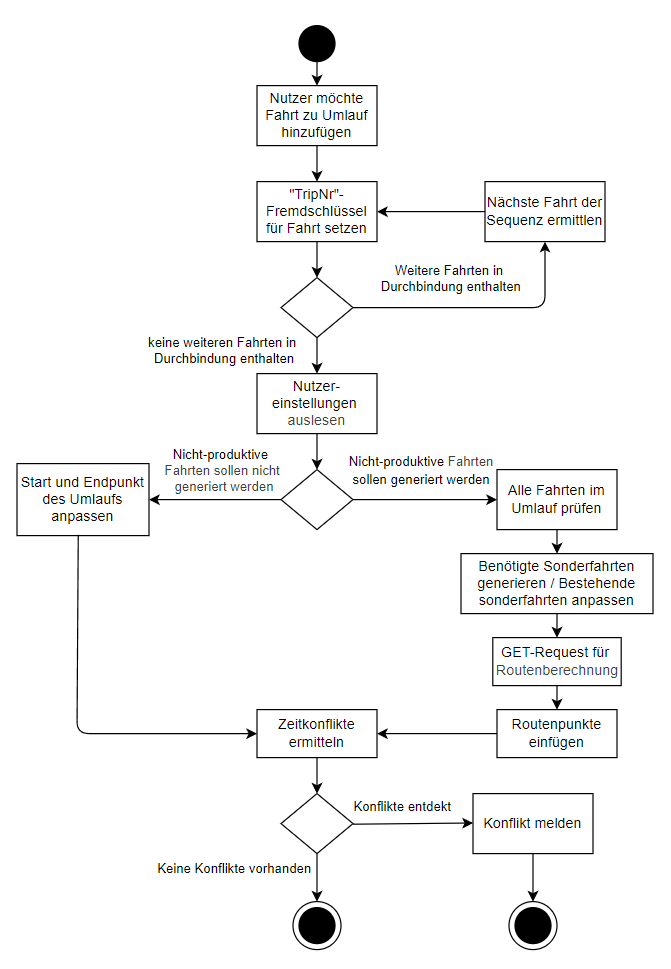
\includegraphics[width=0.8\textwidth]{Ablauf.png}
        \caption{Beziehungen von Umläufen und Fahrten}
        \label{fig:Ablauf}
    \end{figure}

     
\section{"ITCS"}\label{sec:itcs-design}
    Das Projekt \emph{"ITCS"} beinhaltet die SQL-Scripts die alle Änderungen an der Datenbank dokumentierten, um das Schema auf einer neuen Datenbank reproduzieren zu können. 
    Jedem dieser Scripte wird eine aufsteigende Versionsnummer zugeordnet. Diese Versionsnummer wird beim Aufruf des Scripts in eine eigene Datenbanktabelle eingetragen, um den Stand des Schemas
    eindeutig zu dokumentieren. Im Zuge des Praktikums wurde das Datenbank-Schema um einige neuen Tabellen erweitert und bestehende Tabellen um neue Spalten ergänzt. Das resultierte in
    einigen kleineren Create- und Alter-DDL-Scripten. Beispiele dafür sind die Erstellung einer neuen Tabelle für Sonderhaltepunkte oder das Einführen einer neuen Spalte bei Mandanten 
    die abspeichert welche Arten von Sonderfahrten für diese generiert werden sollen.

    Wie bereits erwähnt, liegt der Fokus des Projekts eigentlich auf den Import- und Export-Routinen. Diese werden verwendet, um Daten aus anderen Datenbanken oder Dateien mit dem 
    \emph{VDV-452}~\cite{VDV452} konformen \emph{"x10"}-Format in die ITCS-Datenbank zu importieren. Meist umfasst der Datentransfer eine neue Version des Fahrplans.
    Dieses Projekt nutzt jedoch nicht das \gls{efc} für den Zugriff auf Datenbanken, sondern verwendet die \emph{System.Data.SqlClient}-Bibliothek.
    Diese ist eine .NET-Bibliothek, die es ermöglicht, SQL-Server-Datenbanken zu verwalten 
    und zu manipulieren. Mithilfe dieser wurden ein eigener Datenbaken-Manager und ein attributbasiertes "Object-Relational Mapping" implementiert. Da alle Klassen dadurch von den 
    Basis-Klassen \texttt{Entity} und \texttt{VersionedEntity} erben, ist dieses Vorgehen eher restriktiv, jedoch auf den spezifischen Anwendungsfall optimiert.
    
    Die Routinen für den Import und Export lesen dann Daten aus einer Quelle, speichern diese im Arbeitsspeicher zwischen und schreiben sie dann entweder in eine Datenbank oder in eine Datei.
    Oftmals müssen die Daten dabei angepasst werden, da Quelle und Ziel unterschiedliche Datenschemen verwenden. 

    Der Datenbank-Zugriff und die Routinen wurden jedoch schon vor dem Praktikum implementiert und musste daher nur noch geringfügig angepasst werden, wenn neue Tabellen oder Spalten hinzugefügt wurden.
    Die Anpassungen beschränkten sich dabei auf das Hinzufügen von neuen Methoden im Datenbank-Manager und neuer Domain-Model-Klassen, die die neuen Tabellen repräsentieren.
    
    Im Praktikum wurde dieses Projekt hauptsächlich verwendet, um Methoden, deren Logik in anderen Projekten wiederverwendet werden können sollte, zu implementieren. 
    Dies umfasst beispielsweise die Generierung von Daten wie Metadaten für Sonderfahrten. Wenn die Koordinaten der Sonderhaltepunkte für die neu generierte Sonderfahrt definiert wurden,
    sollte ein \emph{HTTP}-Request an eine externe API gesendet werden, um berechnete Strecke inklusive Fahrtbeschreibung in Form von Wendepunkten zu erhalten. Diese 
    Informationen wird dann aus der \emph{JSON}-Response extrahiert und in der Datenbank gespeichert. Fahrtzeit und -länge werden 
    später für die Ermittlung von Konflikten zwischen Fahrten in Umläufen benötigt. Die Streckenbeschreibung wird für eine 
    visuelle Darstellung der Fahrt benötigt. Diese ist aber nicht mehr Teil des Praktikums.
